\documentclass[crop]{standalone}

\usepackage{amsmath}

\usepackage[dvipsnames]{xcolor}
\usepackage{tikz}

\usetikzlibrary{shapes,decorations,arrows,calc,arrows.meta,fit,positioning}
\tikzset{
    -latex,
    node distance =1 cm and 1 cm,
    inner sep =0.15cm,
    semithick,
    O/.style ={rounded rectangle, draw, minimum width = 0.7 cm},
    U/.style ={rounded rectangle, draw, minimum width = 0.7 cm, dashed},
    fontscale/.style = {font=\huge}
}

\begin{document}


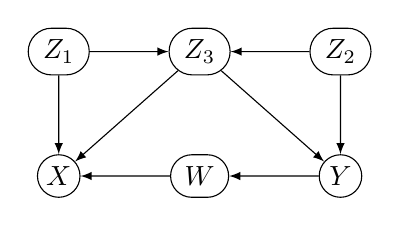
\begin{tikzpicture}
  \node[O] (z1) at (0,0) {$Z_1$};
  \node[O] (z3) [right =of z1] {$Z_3$};
  \node[O] (z2) [right =of z3] {$Z_2$};
  \node[O] (w) [below =of z3] {$W$};
  \node[O] (x) [below =of z1] {$X$};
  \node[O] (y) [below =of z2] {$Y$};
  \path (z1) edge (z3);
  \path (z2) edge (z3);
  \path (z3) edge (x);
  \path (z3) edge (y);
  \path (z1) edge (x);
  \path (z2) edge (y);
  \path (y) edge (w);
  \path (w) edge (x);

\end{tikzpicture}


\end{document}
